\section{Benchmark NIST-10 "Interior Line Singularity"}
\label{sec:bench-10}

This is another example with anisotropic solution that is suitable for testing
anisotropic element refinements.
The equation solved is a Poisson equation

\begin{equation} \label{interior}
-\Delta u = f
\end{equation}
in the domain $\Omega = (-1, 1)^2$, equipped with a zero
Neumann boundary condition on left edge, Dirichlet boundary conditions given by the
exact solution on the rest of the boundary.

The exact solution
\begin{equation}\label{exact-nist-10-1}
u(x,y) = \cos(Ky)\ \ \ \mbox{for}\ x \le 0
\end{equation}
\begin{equation}\label{exact-nist-10-2}
u(x,y) = \cos(Ky) + x^{\alpha}\ \ \ \mbox{for}\ x > 0
\end{equation}
where $K$ and $\alpha$ are real constants.
The right-hand side $f$ is calculated by inserting
(\ref{exact-nist-10-1}) and (\ref{exact-nist-10-2}) into (\ref{wave-front}).
The solution of NIST-10 with $K = \pi/2$ and
$\alpha = 2.01$ is shown in Fig. \ref{fig:sln-nist10}.

\begin{figure}[!ht]
\centering
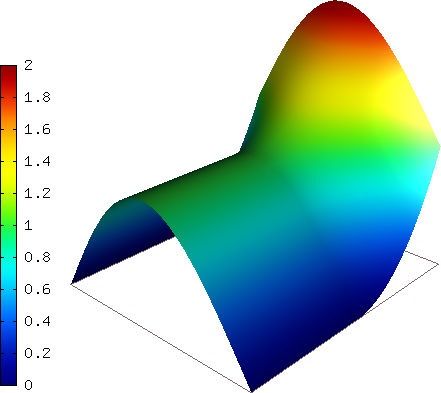
\includegraphics[height=6cm]{nist/nist-10/solution.png}
\caption{The solution to NIST-10 benchmark problem.}
\label{fig:sln-nist10}
\end{figure}
